% -*- TeX:de -*-
\NeedsTeXFormat{LaTeX2e}
\documentclass[12pt,a4paper,titlepage]{article}

%\usepackage[german]{babel} % german text
\usepackage[DIV12]{typearea} % size of printable area
\usepackage[T1]{fontenc} % font encoding
\usepackage[utf8]{inputenc} % probably on Linux

\usepackage{graphicx} % to include images
\usepackage{subfigure} % for creating subfigures
\usepackage{amsmath} % a bunch of symbols
\usepackage{amssymb} % even more symbols
\usepackage{booktabs} % pretty tables
\usepackage{csquotes}

% a floating environment for circuits
\usepackage{float}
\usepackage{caption}

\usepackage[european]{circuitikz}
\ctikzset{voltage/distance from line=.25}% pos. between 0 and 1

\newfloat{circuit}{tbph}{circuits}
\floatname{circuit}{Schaltplan}

% a floating environment for diagrams
\newfloat{diagram}{tbph}{diagrams}
\floatname{diagram}{Diagramm}

\renewcommand{\familydefault}{\sfdefault} % activate to use sans-serif font as default

\sloppy % friendly typesetting

\usepackage{eurosym}
%\usepackage{makeidx}
\usepackage{amsfonts}
\usepackage{mparhack}
\usepackage{array}
\usepackage{tabularx}
\usepackage{minitoc}
\usepackage[colorlinks=true]{hyperref}
\usepackage{epstopdf}
\usepackage{setspace}
\usepackage{csquotes}

\usepackage{pgfplots}
\usetikzlibrary{automata,arrows,chains,shapes.misc,scopes,petri}

\usepackage{csvsimple}
\usepackage{siunitx,array,booktabs}
\usepackage{longtable}
\usepackage[pass]{geometry}


\ctikzset{voltage/distance from node=.5}% in \pgf@circ@Rlen units
\ctikzset{voltage/distance from line=.33}% pos. between 0 and 1
\ctikzset{voltage/bump b/.initial=1.5}%

\begin{document}

\begin{titlepage}

\begin{figure*}[h!]
  \includegraphics[width=8cm]{TULogo_CMYK}
\end{figure*}

\begin{center}
\vspace*{1.3cm}
{\Huge Elektrotechnische Grundlagen der Informatik\\(LU 182.692)\\}
\vspace{1.7cm}
{\LARGE Protokoll der 4. Laborübung: \enquote{Spektren}\\}
\vspace{1.7cm}

% fill in group number and date of lab here
% CHANGE ME!
{\Large Gruppennr.: 10 \hspace{1cm} Datum der Laborübung: 22.06.2017}

% fill in IDs and names here
% CHANGE ME!
\begin{table}[h!]
\centering
\begin{tabular}{|p{3.5cm}|p{3.5cm}|p{6.5cm}|}
\hline \textbf{Matr. Nr.} & \textbf{Kennzahl} & \textbf{Name} \\
\hline
1609418 & 033 535 & GEISELBRECHTINGER Max \\
\hline
1625753 & 033 535 & HAAR Martin \\
\hline
& & \\
\hline
\end{tabular}
\end{table}

\end{center}
\vspace{1.0cm}

\begin{table}[h!]
\begin{tabular}{|l|l|}
\hline \textbf{Kontrolle} & \checkmark \\
\hline Sinus-Signal im Frequenzbereich & \\
\hline Rechteck-Signal im Frequenzbereich & \\
\hline Amplitudenmodulation & \\
\hline Brückengleichrichter & \\
\hline
\end{tabular}
\end{table}

\end{titlepage}
\setcounter{page}{2}

%only sections in tableofcontents, no subsections
\setcounter{tocdepth}{1}
%sets tableofcontents color black
\hypersetup{linkcolor=black}

% start of actual lab protocol
% CHANGE ME!
\tableofcontents
% !TEX root = deckblatt4.tex
\section{Messung eines Sinussignales im Spektralbereich mittels FFT}

\subsection{Aufgabenstellung}
In dieser Aufgabe sollte man sich mit mit der FFT Funktion des Oszilloskops vertraut machen. Hierzu sollte ein einfaches Sinussignal in Zeit und Frequnezbereich gemessen und analysiert werden.

\subsection{Zeitbereich}

\begin{figure}[H]
 \begin{center}
  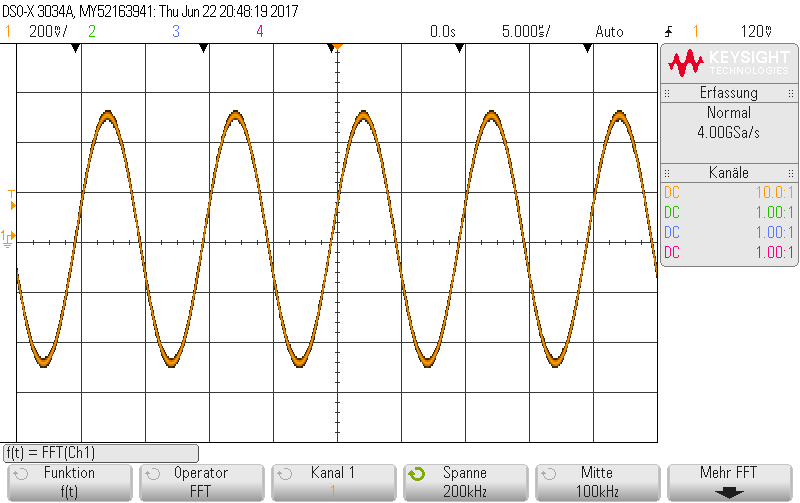
\includegraphics[height=6cm,width=12cm]{OsziBilder/bsp1_time}
 \end{center}
 \caption{Zeitverlauf des Sinussignales, $1V_{PP}$ $100kHz$}
\end{figure}

\subsection{Frequenzbereich}

\begin{figure}[H]
 \begin{center}
  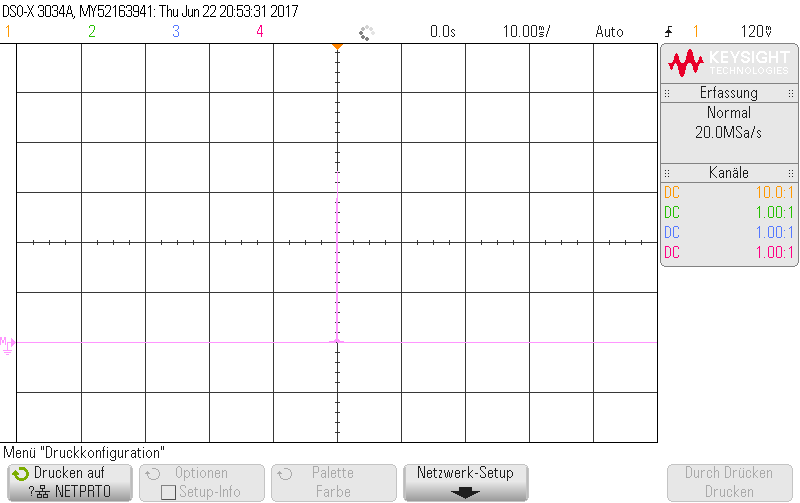
\includegraphics[height=6cm,width=12cm]{OsziBilder/bsp1_Rechteck_RMS}
 \end{center}
 \caption{Spektraldarstellung des Sinussignales, Rechteckfenster $V_{RMS}$}
\end{figure}

\begin{figure}[H]
 \begin{center}
  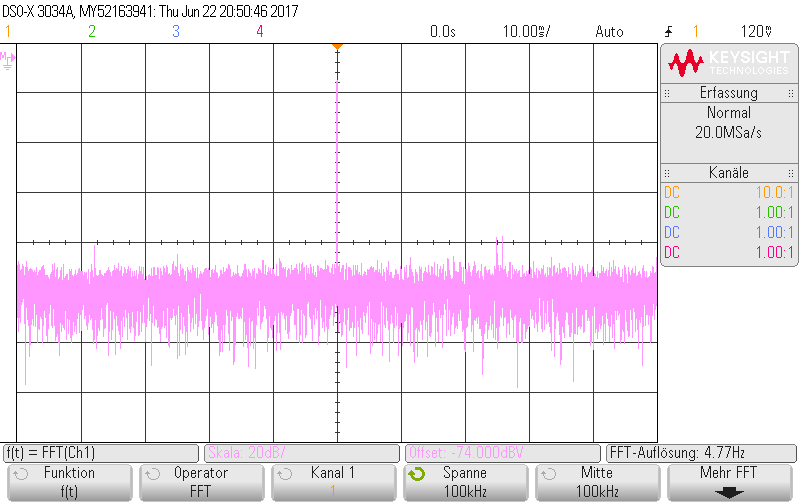
\includegraphics[height=6cm,width=12cm]{OsziBilder/bsp1_Hanning_dB}
 \end{center}
 \caption{Spektraldarstellung des Sinussignales, Hammingfenster $dBV$}
\end{figure}
\noindent
Beide Darstellungen zeigen die Spektrallinie des Sinussignales bei $1kHz$ mit einer Amplitude von $0,5V_P$. In der $dBV$-Skalierung kommen auch die Signale mit kleinerer Amplitude zur geltung, weshalb auch die Störsignale (Rauschen) zu sehen sind.\\
Um durch die FFT ein sauberes Spektrum zu erlangen, müssen verschiedene Parameter angepasst werden. So ist ist die Abtastrate (Horizontalablenkung) ausschlaggebend für die korrekte Aufzeichnung des Signales (Aliasing- Foldingeffekt). Der Frequenzbereich wird so gewählt, dass
die einezelnen Spektralkomponent gut zu erkennen sind und die benötigte Bandbreite dargestellt wird.\\

\newpage
\subsection{Fensterfunktionen}

Die Fensterfunktionen werden nach den Kriterien, minimaler Leckeffekt, Amplituden- und Frequenzgenauigkeit gewählt. Da es keine optimale Lösung gibt, die alle drei Anforderungen erfüllt, wird
die Fensterfunktion abhängig von der Problemstellung gewählt.\\
Das Oszilloskop bietet vier Verschiedenen Fensterfunktion:\\
\begin{itemize}
 \item Rechteckfenster: hoher Leckeffekt, hohe Frequenzgenauigkeit\\
 \item Hammingfenster: gut für kontinuierliche Signale\\
 \item Flache Oberseite Fenster: hohe Amplituden genauigkeit, niedrige Frequenzgenauigkeit \\
 \item Blackman-Harris-Fenster:  hohe Amplituden genauigkeit, niedrige Frequenzgenauigkeit\\
\end{itemize}
Für die weiteren Anwendungen der FFT wurde hauptsächlich das Hammingfenster verwendet, da es einen guten Kompromiss
zwischen den drei geforderten Eigenschaften darstellt.\\

% !TEX root = deckblatt4.tex
\section{Messung eines Rechtecksignals}
\subsection{Aufgabenstellung}
Hier sollte ein Rechtecksignal in Zeit und Frequnenzbereich gemessen werden und anschlie\ss{}end die Ergebnisse erl\"autert werden

\subsection{Vorbereitung \& Messaufbau}
Es wurde mit dem Frequnezgenerator ein Rechtecksingal mit einer Amplitude von $1V_{pp}$ und einer Frequnez von $10kHz$ erzeugt. Der Ausgang des Frequnezgenerators wurde direkt mit dem Tastkopf des Oszilloskops verbunden, es wurde keine Messschaltung aufgebaud.

\begin{figure}[H]
 \begin{center}
  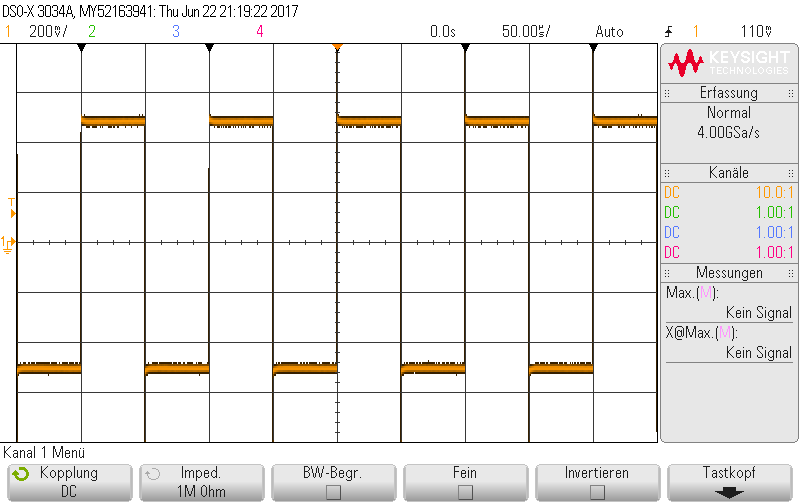
\includegraphics[height=6cm,width=12cm]{OsziBilder/bsp2_time.png}
 \end{center}
 \caption{Rechteckspannung $1V_{pp}$, $10kHz$}\label{bsp2_time}
\end{figure}
\noindent
In Abbildung \ref{bsp2_time} ist, dass Rechtecksignal, welches zur Messung verwendet wurde im Zeitbereich zu sehen. \\
\newpage

\subsection{FFT}
In dieser Messung wurde das Hanning-Fenster verwendet, da dies ein sehr einfaches und g\"angiges Fenster ist.

\begin{figure}[H]
 \begin{center}
  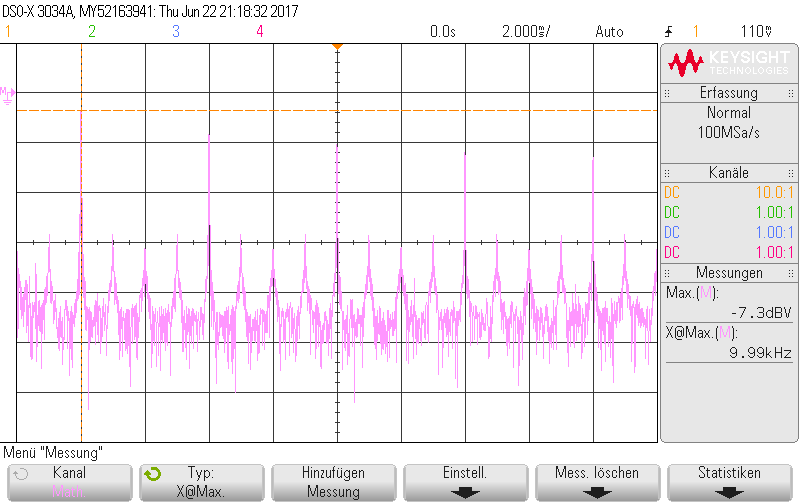
\includegraphics[height=6cm,width=12cm]{OsziBilder/bsp2_Hanning_dB.png}
 \end{center}
 \caption{Rechteckspannung $1V_{pp}$, $10kHz$}\label{bsp2_dB}
\end{figure}
\noindent

\begin{figure}[H]
 \begin{center}
  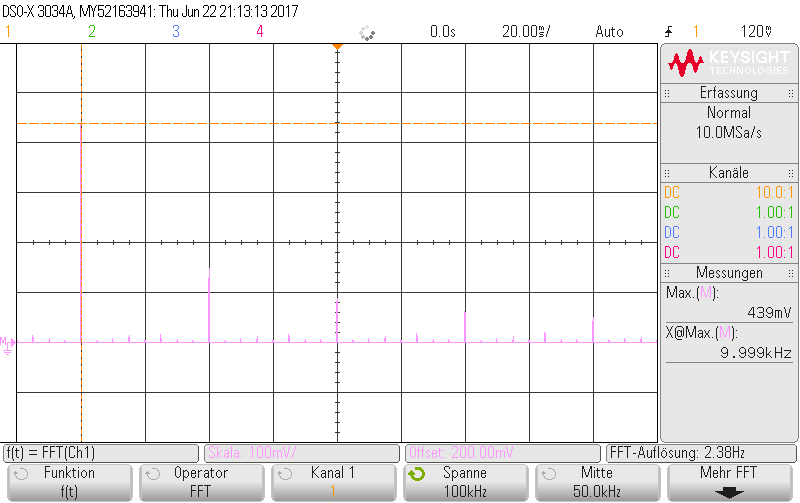
\includegraphics[height=6cm,width=12cm]{OsziBilder/bsp2_Hanning_RMS_Cursor.png}
 \end{center}
 \caption{Rechteckspannung $1V_{pp}$, $10kHz$}\label{bsp2_rms}
\end{figure}
\noindent
In den beiden Abbildungen \ref{bsp2_dB} \& \ref{bsp2_rms} sind die Spektren des oben gezeigten Rechtecksignals zu sehen. In Abbildung \ref{bsp2_dB} wurde f\"ur die y-Achse eine logarithmische ($dB$) und in Abbildung \ref{bsp2_rms} eine lineare Skalierung gewählt. \\
In den beiden Abbildungen ist der Vorteil der dB - Skalierung deutlich zu erkennen. W\"ahrend in Abbildung \ref{bsp2_dB} die Amplitude bei $90kHz$ nur um etwa $10dB$ kleiner als die der Grundfrequnez ist, so ist diese in der linearen Darstellung schon verschwindend gering. \newpage \noindent
Wie erwartet stechen bei einem Symetrischen Rechteck alle Ungeraden Vielfachen der Grundfrequenz hervor. Warum dies so ist l\"asst sich mathematisch leicht begr\"unden \\ \\
Eine Rechteckfunktion ist folgenderma\ss{}en definiert:
\begin{center}
    $f(t) = \left\{\begin{array}{ll}
            1        \hspace{1.5cm} 0\leq t < \pi\\
            0        \hspace{1.5cm} \pi \leq t < 2\pi
            \end{array}\right.$
\end{center}
\noindent
Diese Funktion ist Rotationssymetrisch und somit sind alle cos-Anteile 0
\begin{center}
  \begin{align*}
    a_0 &= \frac{1}{2\pi}\int_0^{\pi} 1 dt = \frac{1}{2} \\
    b_n &= \frac{1}{2\pi}\int_0^{\pi} sin(nt) dt \\
    b_n &= \frac{1}{2\pi} \left[ -\frac{cos(n\pi)}{n} + \frac{1}{n} \right] = -\frac{1}{2n\pi} \left[ (-1)^n - 1  \right] \\
    b_n &= \left\{\begin{array}{ll}
            0              \hspace{1.5cm} \text{f\"ur n gerade}\\
            \frac{1}{n\pi} \hspace{1.3cm} \text{f\"ur n ungerade}
            \end{array}\right. \\
  \end{align*}
\end{center}
\noindent
Am Ergebnis der Fourierreihe ist zu sehen, dass die Spektralanteile f\"ur alle geraden Vielfachen der Grundfrequnez 0 Ergeben, und die Amplituden der ungeraden Anteile mit dem Faktor $\frac{1}{n\pi}$ kleiner werden.

\begin{figure}[H]
  \begin{center}
    \begin{tabular}{|c|c|} \hline
    $f_g=10kHz$ & $439mV$ \\ \hline
    $3*f_g$ & $147,11mV$ \\ \hline
    $5*f_g$ & $90,77mV$ \\ \hline
    $7*f_g$ & $62,60mV$ \\ \hline
    \end{tabular}
  \end{center}
  \caption{Messwerte der Hauptkomponente und der ersten 3 Nebenkomponenten}
\end{figure}
\noindent
In obiger Tabelle sind die Amplituden zu der Grundfrequenz und den ersten drei ungeraden Vielfachen gemessen worden. Man kann sehr gut erkennen, dass die Werte hyperbolisch abnehmen.

% !TEX root = deckblatt4.tex
\section{Amplitudenmodulation}
\subsection{Aufgabenstellung}
Es sollte ein Nutzsignal auf ein Hochfrequenztes Tr\"agersignal aufmoduliert werden und anschlie\ss{}end im Frequneznbereich gemessen werden. Des weiteren mussten Berechneungen durchgef\"uhrt werden und mit den Messergebnissen verglichen werden.

\subsection{Brechnungen}
\begin{center}
  \begin{align*}
    U_{AM}(t) &= \frac{U_0 + U_{info}(t)}{U_0 + \hat{U}_{info}} * U_{carrier}\\
    U_{carrier}(t) &= \hat{U}_{carrier}+cos(\omega_c t)\\
    U_{info} &= \hat{U}_{info} * f_{info}(t)
  \end{align*}
\end{center}

% !TEX root = deckblatt4.tex
\section{Br\"uckengleichrichter}
\subsection{Aufgabenstellung}
In dieser Aufgabe musste ein Br\"uckengleichrichter aufgebaut werden und Zeit- und Frequenzmessungen durchgef\"uhrt werden. Des weiteren sollte eine Fourierreihe Berechnet und mit den Ergebnissen verglichen werden.

\subsection{Messschaltung}
\begin{figure}[ht!]
  \begin{center}
    \begin{circuitikz}\draw
    (0,0) to[sI] (0,6) to[Do] (7,6) to[R={$R_1$}{$=1M$}](7,0) to[Do] (0,0)
    (2,0) to[short, *-] (2,4) -- (2.5,4) to[Do] (4.5,4) -- (5,4) to[short,-*] (5,6)
    (5,0) to[short, *-] (5,2) -- (4.5,2) to[Do] (2.5,2) -- (1.5,2) to[short, -*] (1.5,6)
    (0,0) node[ground]{};
    \draw[-latex] (8.5,6) -- (7.3,6);
    \draw (9.6,6) node[] {Kanal 1};
    \draw[-latex] (8.5,0) -- (7.3,0);
    \draw (9.6,0) node[] {Kanal 2};
    \draw (3.5,7) node[] {1N4148};
    \end{circuitikz}
  \end{center}
  \caption{Messschaltung}\label{bsp4_circ}
\end{figure}
\noindent
In Abbildung \ref{bsp4_circ} ist der Br\"uckengleichrichter, welcher f\"ur die nachfolgenden Messungen verwendet wird zu sehen. Der Gelichrichter besteht aus vier Dioden (1N4148). Die Ausgangsspannung am Widerstand $R_1$ kann nicht einfach abgegriffen werden da sonst ein Teil der Schaltung \"uber die Masse des Oszilloskops kurgeschlosswern werden w\"urde. Aus diesem Grund wurde mit 2 Kan\"alen gemessen und die Masse der Tastk\"opfe wurde mit der Masse des Funktionsgenerators an einen Punkt geschalten. Anschlie\ss{}end die Differenz mit der "Math"-Funktion des Oszilloskops berrechnet.

\subsection{Messung im Zeitbereich}
\begin{figure}[H]
 \begin{center}
  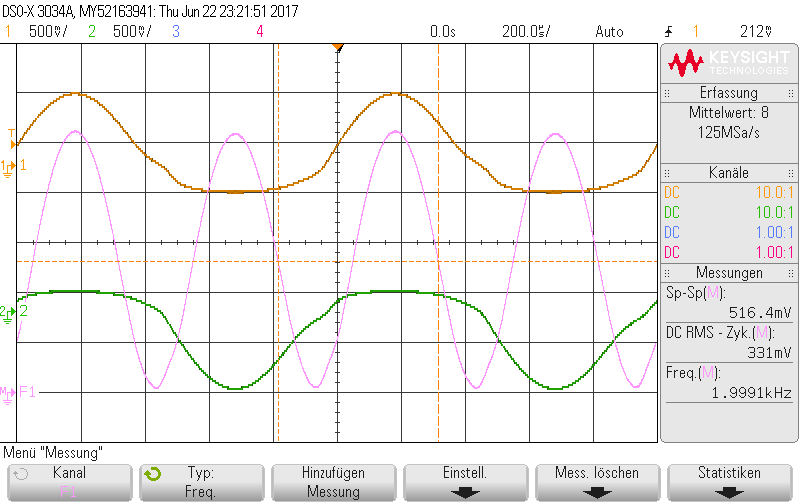
\includegraphics[height=6cm,width=12cm]{OsziBilder/bsp4_sin_time_2Vpp_UeUa.png}
 \end{center}
 \caption{Sinussingal $2V_{pp}$, $1kHz$}\label{bsp4_time2V}
\end{figure}
\noindent

\begin{figure}[H]
 \begin{center}
  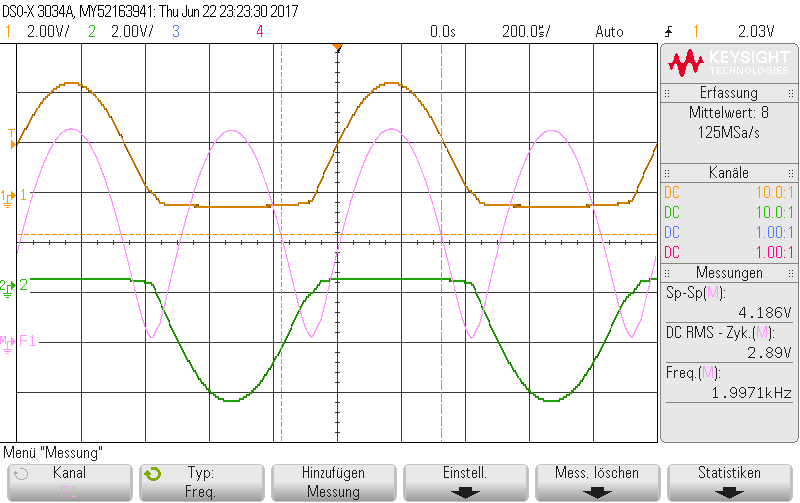
\includegraphics[height=6cm,width=12cm]{OsziBilder/bsp4_time_10Vpp_UeUa.png}
 \end{center}
 \caption{Sinussingal $10V_{pp}$, $1kHz$}\label{bsp4_time10V}
\end{figure}
\noindent
In den beiden Abbildungen \ref{bsp4_time2V} und \ref{bsp4_time10V} sind die Zeitsignale zu sehen. Die Differenz der beiden Kan\"ale ergibt den Gleichgereichteten Sinus, dieser hat die Doppelte Frequnez als das Eingangssignal, jedoch den gleichen Effektiefwert.

\subsection{Fouriereihe}
\begin{center}
  \begin{align*}
    |sin(t)| & \text{ ist eine gerade Funktion} \\ \\
    S(f) &= \frac{a_0}{2} + \sum_{n=1}^{\infty} a_n * cos(nt) \\ \\
    \text{Summensatz S8: } & 2sin(\alpha)cos(\beta) = sin(\alpha-\beta)+sin(\alpha+\beta) \\ \\
    a_0 &= \frac{1}{\pi}\int_0^{2\pi} |sin(t)| dt = \frac{2}{\pi}\int_0^{\pi} sin(t) dt = \frac{4}{\pi} \\ \\
    a_n &= \frac{2}{\pi}\int_0^{\pi} sin(t) * cos (nt) dt \\
    a_n &= \frac{1}{\pi}\int_0^{\pi} sin(t - nt) dt +  \frac{1}{\pi}\int_0^{\pi} sin(t + nt) dt\\
    a_n &= -\frac{1}{\pi} \left[ \frac{cos(\pi(1-n))}{1-n} + \frac{cos(\pi(1+n))}{1+n} \right] \\
    a_n &= -\frac{1}{\pi} \left[ \frac{-(-1)^n-1}{1-n} + \frac{-(-1)^n-1}{1+n} \right] \\
    a_n &= \frac{1}{\pi} \left[ \frac{(-1)^n+1}{1-n} + \frac{-(-1)^n+1}{1+n} \right] \\
    a_n &= \frac{2((-1)^2+1)}{\pi(1-n^2)} \\ \\
    a_n &= \left\{\begin{array}{ll}
            0                     \hspace{2.5cm} \text{f\"ur n ungerade}\\
            \frac{4}{\pi(1-n^2)} \hspace{1.5cm} \text{f\"ur n gerade}
            \end{array}\right.
  \end{align*}
\end{center}

\subsection{FFT}
\begin{figure}[H]
 \begin{center}
  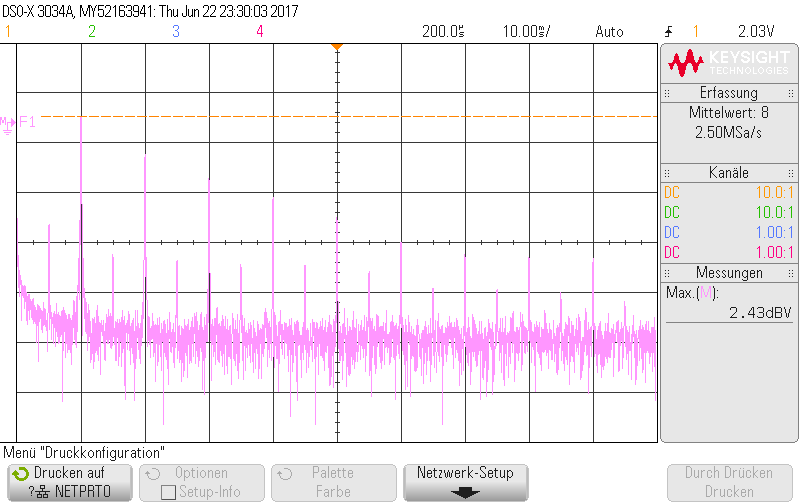
\includegraphics[height=6cm,width=12cm]{OsziBilder/bsp4_sin_fft_10Vpp_dB.png}
 \end{center}
 \caption{Sinussingal $2V_{pp}$, $10kHz$}\label{bsp4_fft}
\end{figure}
\noindent
Genau wie in den Berechnungen ist in dieser Messung zu erkennen, dass jeder zweite Frquenzanteil mit quasi 0 ergibt (ca. $-30dB$) und die Amplituden mit steigender Frequnez rasch kleiner werden.

\begin{figure}[H]
  \begin{center}
    \begin{tabular}{|c|c|} \hline
    $U_0$ & $1,325V$ \\ \hline
    $U_1$ & $231,25mV$ \\ \hline
    $U_2$ & $75mV$ \\ \hline
    $U_3$ & $31,25mV$ \\ \hline
    $U_4$ & $12,2mV$ \\ \hline
    \end{tabular}
  \end{center}
  \caption{Messwerte der f\"unf gr\"o\ss{}ten Spektralen Komponenten}
\end{figure}
\noindent


\end{document}
